%infinitely branching :(
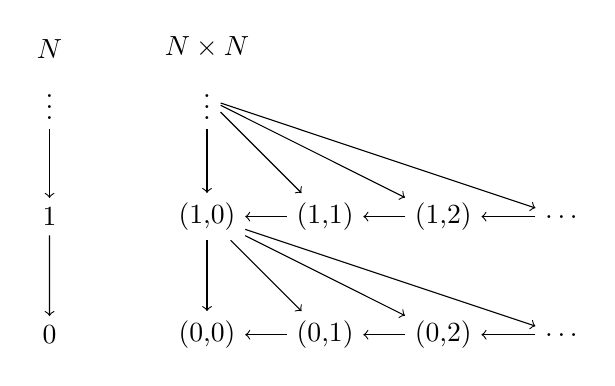
\begin{tikzpicture}[node distance=1.5cm,->,level/.style={level distance = 1.5cm},tree/.style = {align=right}] 
\node [label=above:$\mathbb{N}$] at (0,0) {$\vdots$} 
	child{ node {1}
		child{ node {0}
		}
	};
\node [label=above:$\mathbb{N\times N}$] (a) at (2,0) {$\vdots$}
	child{ node (b1) [below of = a] {(1,0)}
		child{ node (c1) [below of = b1] {(0,0)}	}
		child{ node (c2) [right of = c1] {(0,1)}	}
		child{ node (c3) [right of = c2] {(0,2)}	}
		child{ node (c4) [right of = c3] {$\dots$}	}
	}
	child{ node (b2) [right of = b1] {(1,1)}	}
	child{ node (b3) [right of = b2] {(1,2)}	}
	child{ node (b4) [right of = b3] {$\dots$}	}
	;
	\draw (b2) to (b1);
	\draw (b3) to (b2);
	\draw (b4) to (b3);
	\draw (c2) to (c1);
	\draw (c3) to (c2);
	\draw (c4) to (c3);
\end{tikzpicture}\\
$\mathbb{N}\rightarrow$ finitely branching.\\
$\mathbb{N\times N}\rightarrow$ infinitely branching.\\
Assume there exits a bijective mapping $B:\mathbb{N\times N}\to\mathbb{N}$ such that 
\begin{align*}
(a,b)<_{lex}(c,d) \textbf{ iff } B((a,b))<B((c,d))
\end{align*}holds.
Let $B((1,0))=k$ and consider the increasing chain $(0,0)<_{lex}\dots<_{lex}(0,k)<_{lex}(1,0)$. This chain has $k+2$ elements, the pigeon principle implies 